\documentclass{beamer}
%\usetheme{Copenhagen}
%\usetheme{Boadilla}
\usepackage{geometry}                % See geometry.pdf to learn the layout options. There are lots.
\usepackage{graphicx}
\usepackage{amssymb}
\usepackage{beamerthemeshadow}
 \usepackage{feynmp}
 \usepackage{textpos}
 \usepackage{biblatex}
 \usepackage{bbold}
  \usepackage{ulem}
 \bibliography{foo}
  \DeclareGraphicsRule{*}{mps}{*}{} 
  % figures
  
 % \logo{
\includegraphics[height=1.2cm]{lhcblogo.jpg}\vspace{220pt}}
  
  
\usepackage{caption}
\usepackage{subfig}
\newcommand{\Lagr}{\mathcal{L}}
\setbeamertemplate{itemize item}{\scriptsize\raise1.25pt\hbox{\donotcoloroutermaths$\blacktriangleright$}}
\setbeamertemplate{itemize subitem}{\tiny\raise1.5pt\hbox{\donotcoloroutermaths$\square$}}
\setbeamertemplate{itemize subsubitem}{\tiny\raise1.5pt\hbox{\donotcoloroutermaths$\blacktriangleright$}}
\setbeamertemplate{enumerate item}{\insertenumlabel.}
\setbeamertemplate{enumerate subitem}{\insertenumlabel.\insertsubenumlabel}
\setbeamertemplate{enumerate subsubitem}{\insertenumlabel.\insertsubenumlabel.\insertsubsubenumlabel}
\setbeamertemplate{enumerate mini template}{\insertenumlabel}
\begin{document}
{


\title[ Update on search for $\Lambda_{b} \rightarrow p \mu \nu$ \hspace{2em}\insertframenumber/
\inserttotalframenumber]{Update on search for $\Lambda_{b} \rightarrow p \mu \nu$}
\author[William Sutcliffe]{
\includegraphics[height=1cm,width=1.5cm]{lhcblogo.jpg} \\ William Sutcliffe}

\date{\today}


 \frame{\titlepage

} 

\addtobeamertemplate{frametitle}{}{%
\begin{textblock*}{100mm}(.85\textwidth,-1cm)

\includegraphics[height=1cm,width=1.5cm]{lhcblogo.jpg}
\end{textblock*}}

 %%%%slide 1

% \frame{\frametitle{Outline} 
%\begin{enumerate}
%\setlength{\itemsep}{10pt}
%\item Background and motivation.
%\item Previous measurements.
%\item $V_{ub}$ with LHCb
%\item Initial generator level study
%\end{enumerate}
%}




\frame{\frametitle{Table of contents}\tableofcontents} 

\section{Context and Motivation}
 \frame{
 \frametitle{Current Status of $|V_{ub}|$}
 \begin{itemize}
  \item \normalsize{Semi-Leptonic B Decays:}
   \end{itemize}
   \hspace{1.cm} \footnotesize{Inclusive ($\bar{B} \rightarrow X_{u} l \bar{\nu}_{l}$)} \hspace{1cm}  \footnotesize{Exclusive ($\bar{B}_{0} \rightarrow \pi^{+} l \bar{\nu}_{l}$)}
    \begin{center} 
    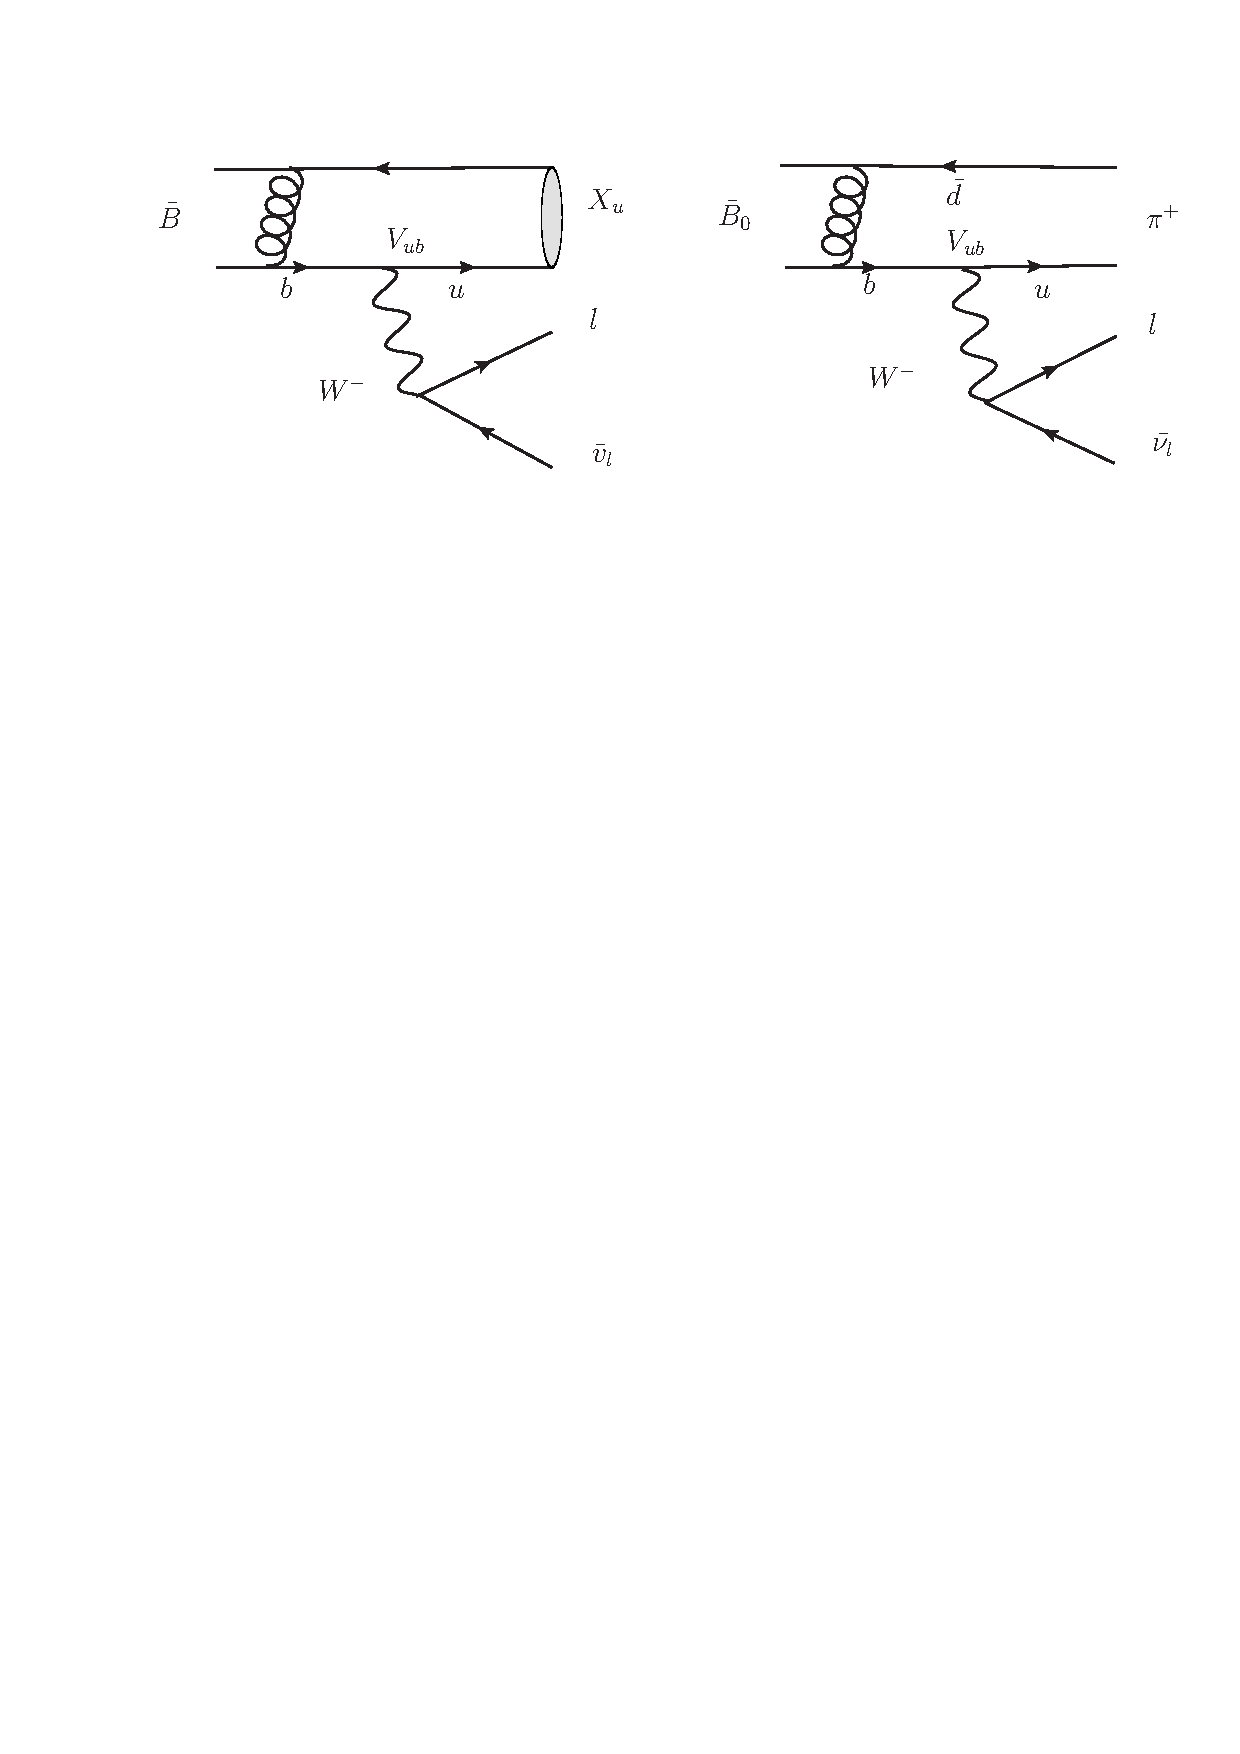
\includegraphics[trim = 15mm 215mm 0mm 25mm, clip, width=8cm]{incl_ex_feyn.pdf} 
        \end{center}
        \hspace{1.cm} \footnotesize{$|V_{ub}| = (4.41 \pm 0.15 ^{+ 0.15} _{-0.17}) \times 10^{-3}$} \hspace{0.3cm} \footnotesize{$|V_{ub}| = (3.23 \pm 0.31) \times 10^{-3}$}
  
  \vspace{0.1cm}
       \begin{itemize}
  \item \normalsize{Leptonic B decays ($B^{+} \rightarrow \tau^{+} \nu_{\tau}$):}
      \begin{center}
       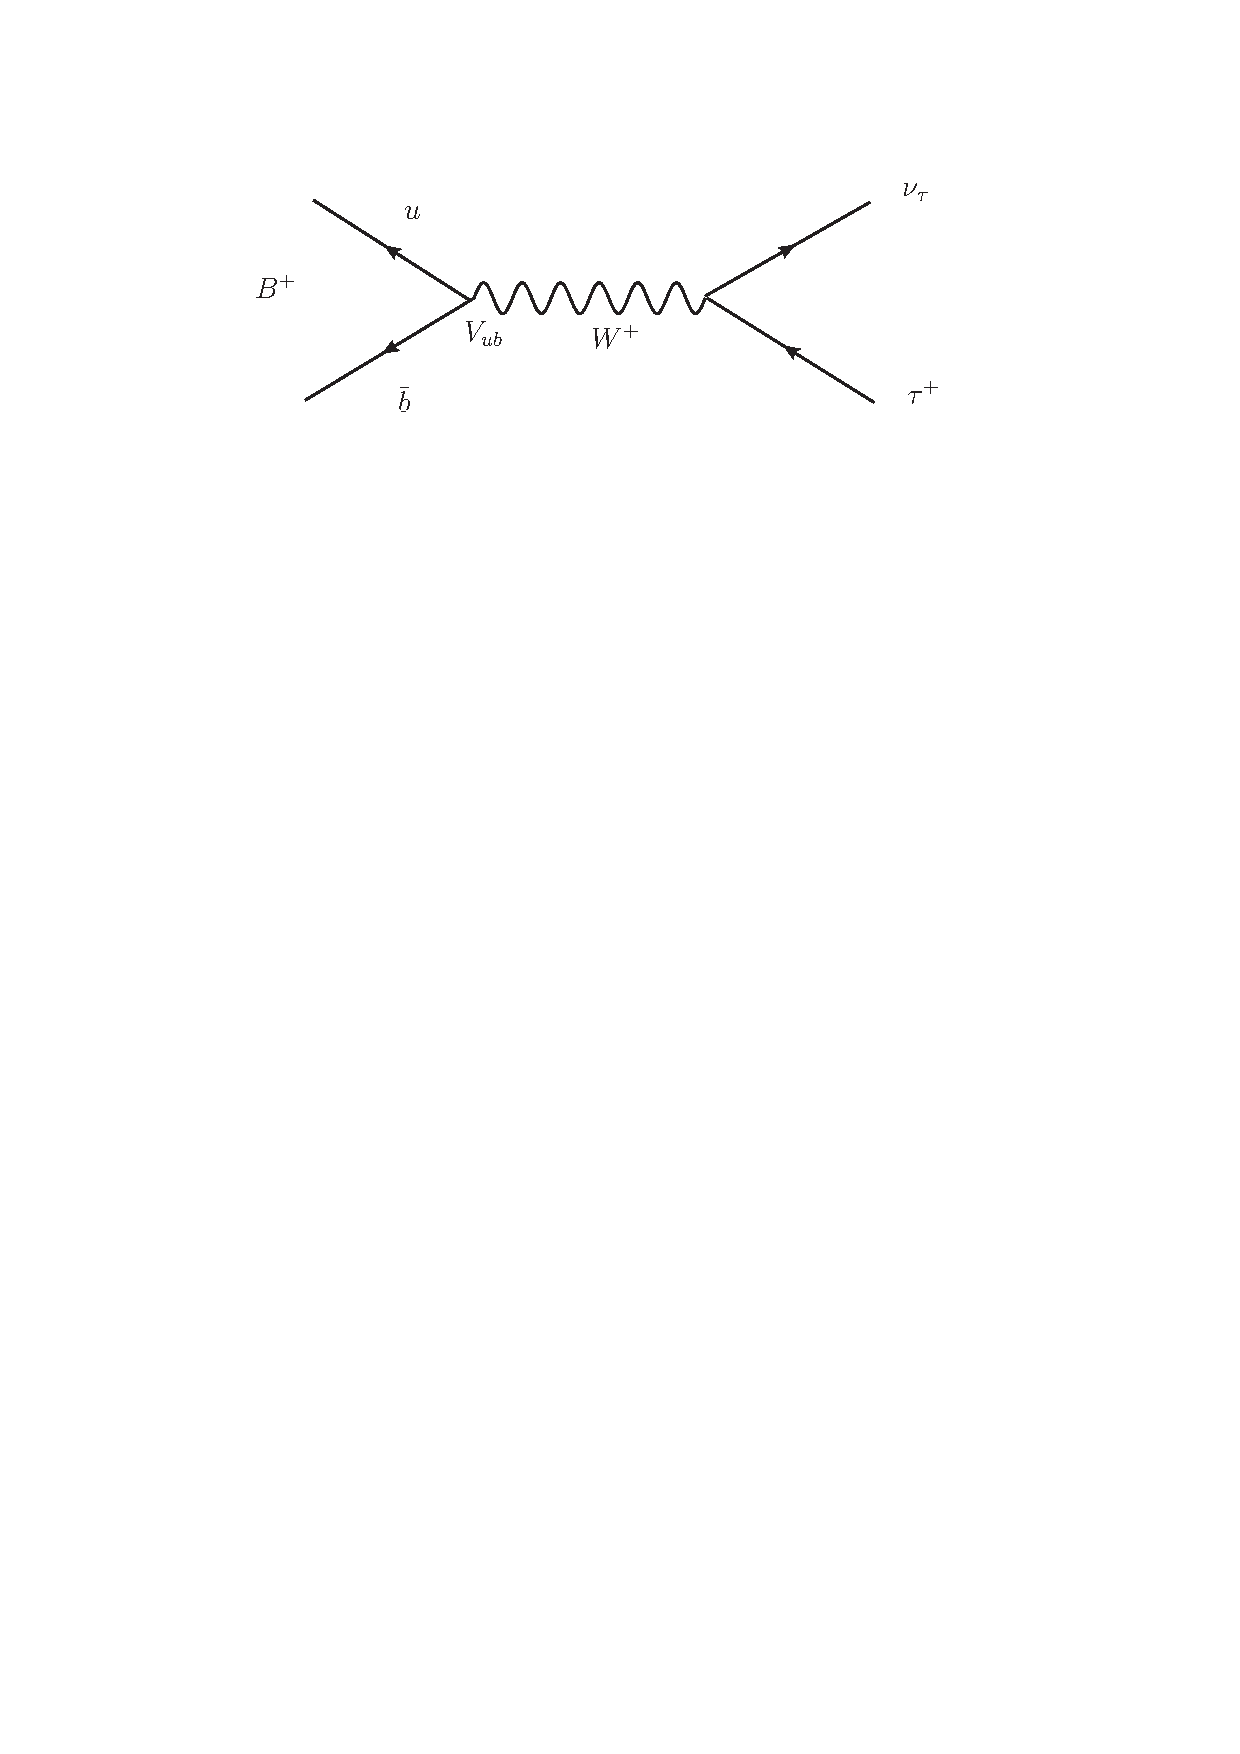
\includegraphics[trim = 15mm 215mm 0mm 30mm, clip, width=8cm]{lepfeyn.pdf} 
       \end{center}
   \end{itemize}
  

}




 \frame{
 \frametitle{$|V_{ub}|$ Constraints on the Unitarity Triangle} 
    \begin{center}
      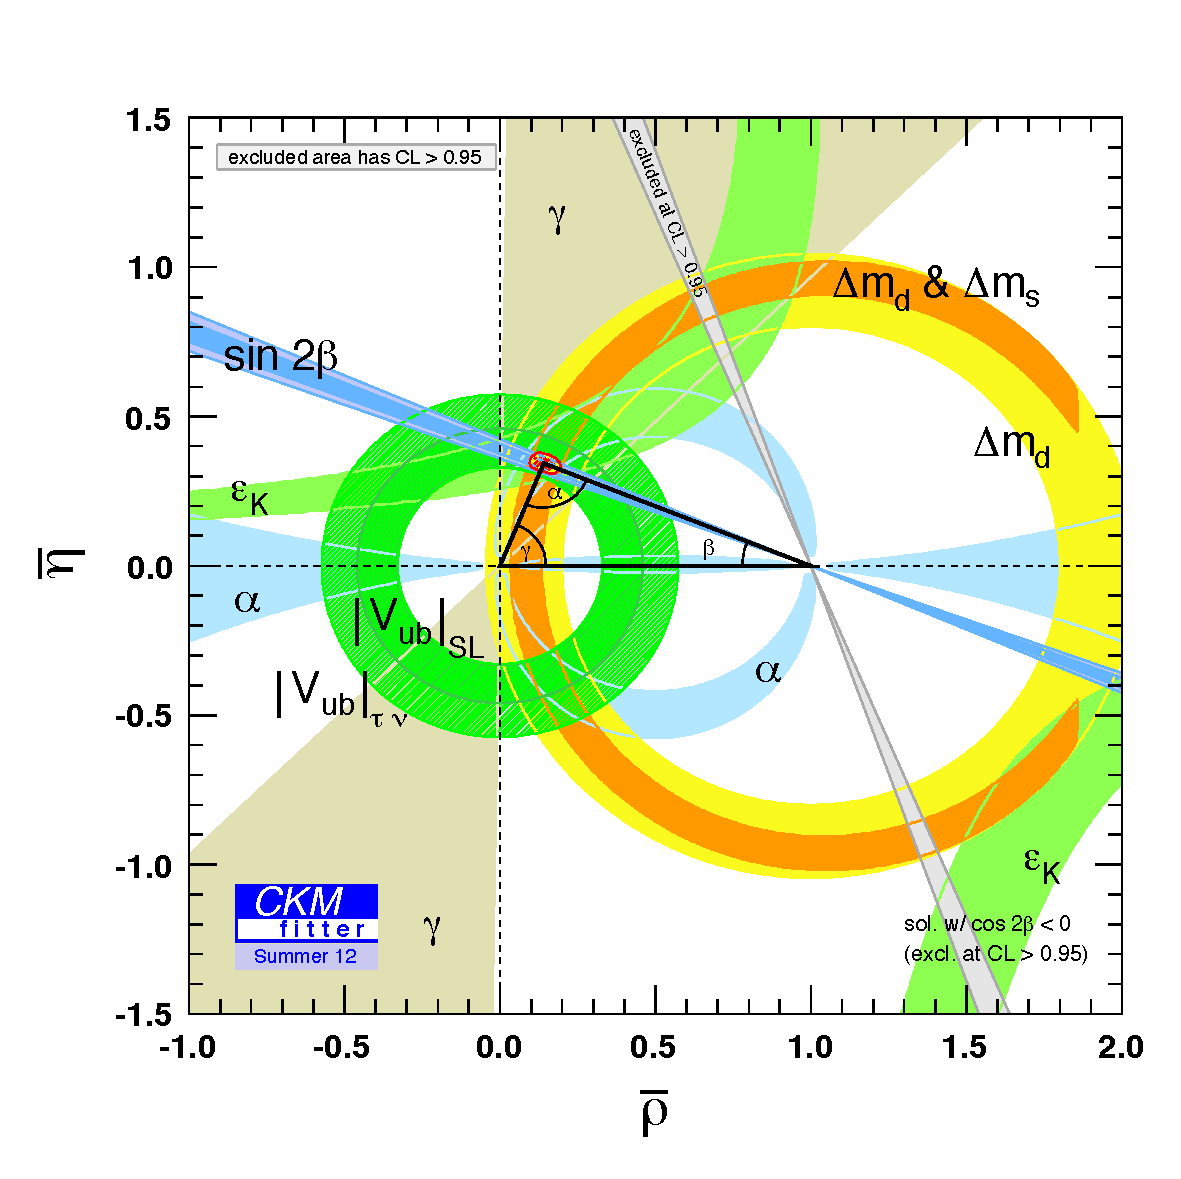
\includegraphics[width=0.6\textwidth]{CKMfit.pdf} 
        \vspace{0.0cm}
   %\hspace{1cm}\tiny{[1] CKMfitter Group, J. Charles et al. ICHEP conference (July 2012)}
  \end{center}
}

\section{Neutrino Reconstruction}
\frame{
\frametitle{Neutrino Reconstruction}
\begin{center}
      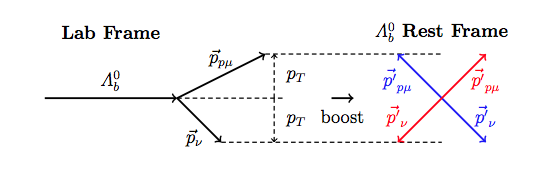
\includegraphics[width=0.6\textwidth]{nureco.png} 
\end{center}
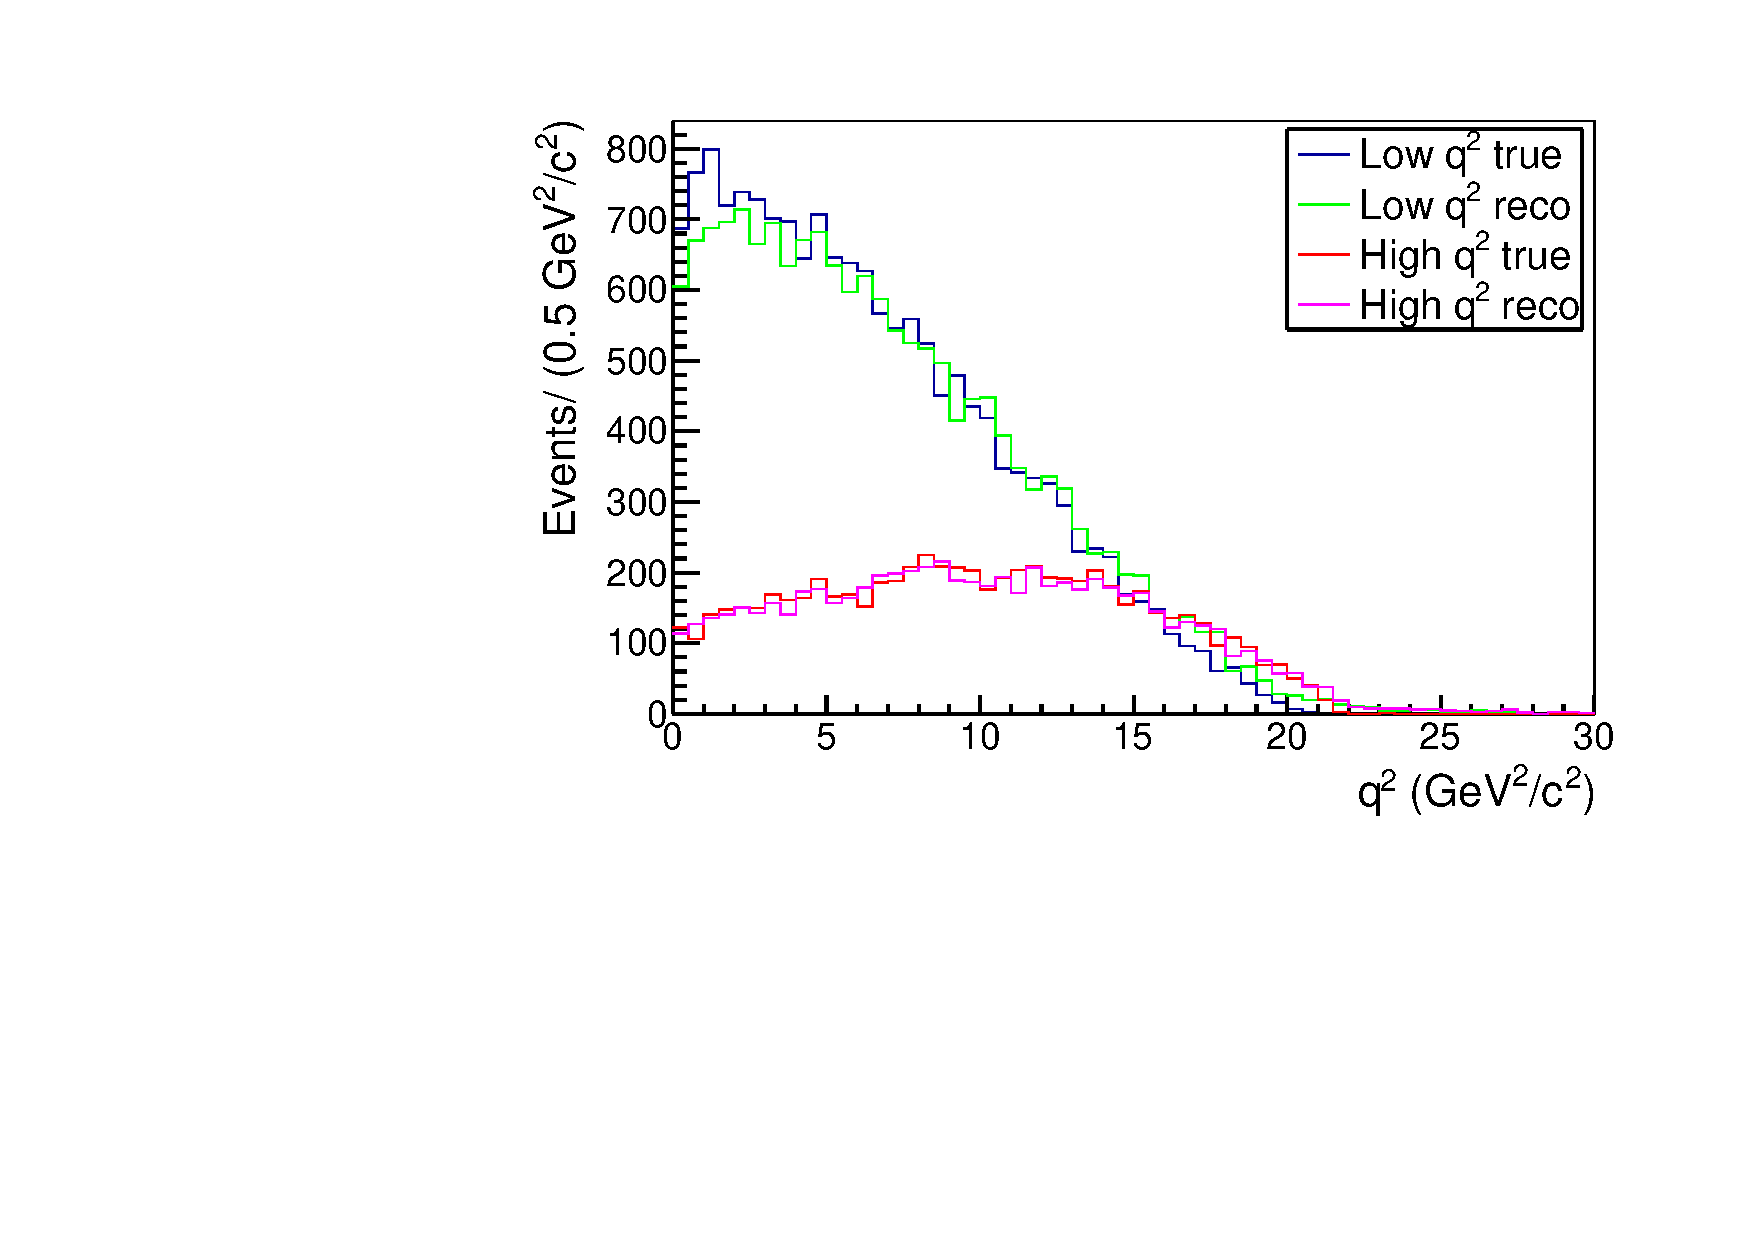
\includegraphics[width=0.5\textwidth]{q2_reco.pdf} 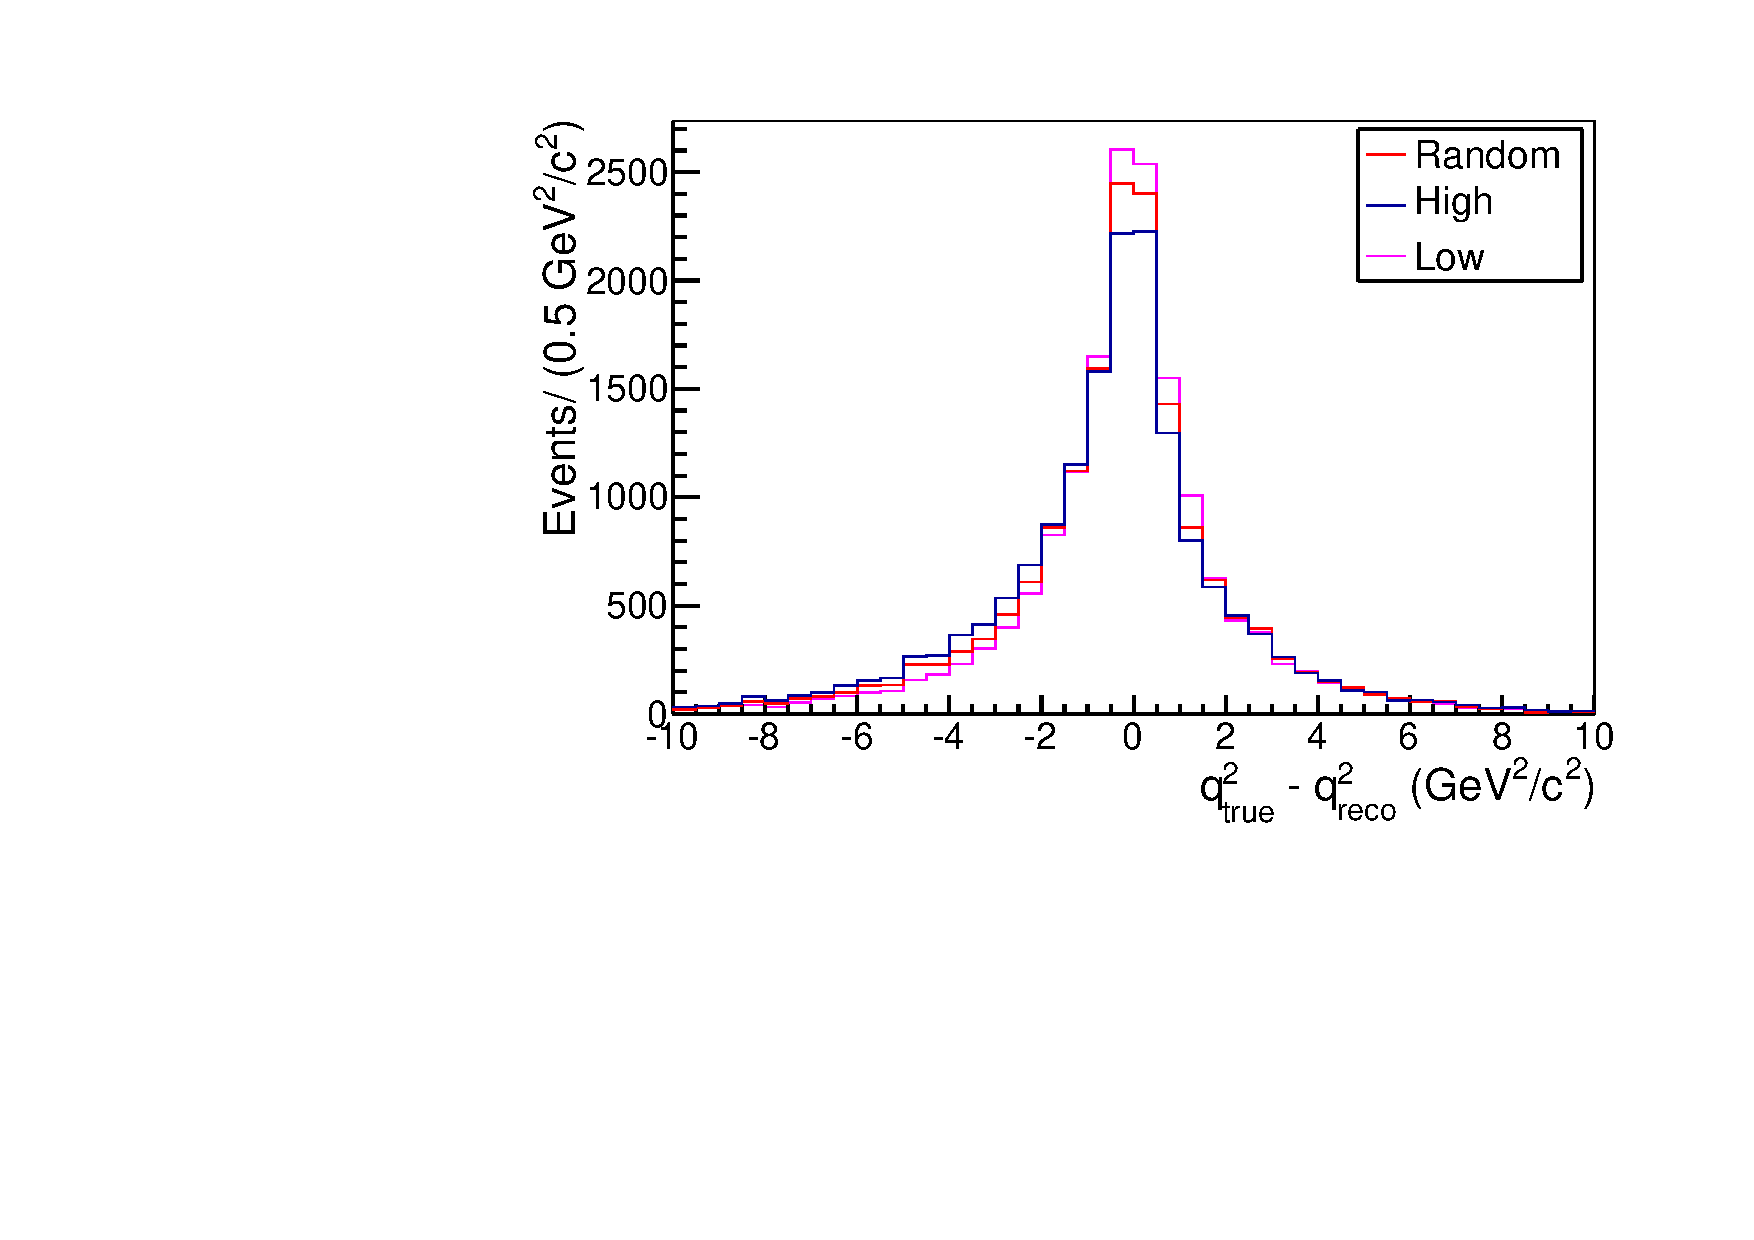
\includegraphics[width=0.5\textwidth]{qdiff.pdf} 
}


      


 
\section{Generator Level Studies}
 \frame{
 \frametitle{Generator Level Studies}
 
\begin{itemize}
 \setlength{\itemsep}{5pt}
\item Generator Level Sample of 3 million inclusive $b\overline{b}$ events.
\item Generator Level Cuts: 
\begin{itemize}
\item Within LHCb acceptance
\item At least one lepton with $p_{\rm{T}}> 1.5$ GeV/c
\end{itemize}
\item Expect this number of events in $\sim$$0.01$pb$^{-1}$ at $\sqrt{s} = 7$ TeV.
\item Search events for protons and muons produced from the decay of the same $B$ hadron.  Ignore protons and muons produced by long-lived intermediaries.
\end{itemize}
    \begin{center}
      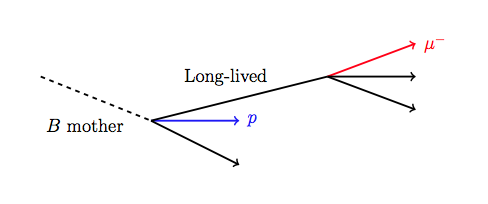
\includegraphics[width=0.6\textwidth]{GL1.png} 
   
   %\hspace{1cm}\tiny{[1] CKMfitter Group, J. Charles et al. ICHEP conference (July 2012)}
  \end{center}

}


\frame{
 \frametitle{}

  \begin{center}
 
\begin{itemize}
  \item Plot opposite sign and same sign $p\mu$ combinations.
  \item Always choose $p$, $\overline{p}$, $\mu^{+}$, $\mu^{-}$  with highest momentum .
  \vspace{0.2cm}
\end{itemize}
 \hspace{1cm}  \uline{Opposite Sign $q^{2}$ Distribution}
      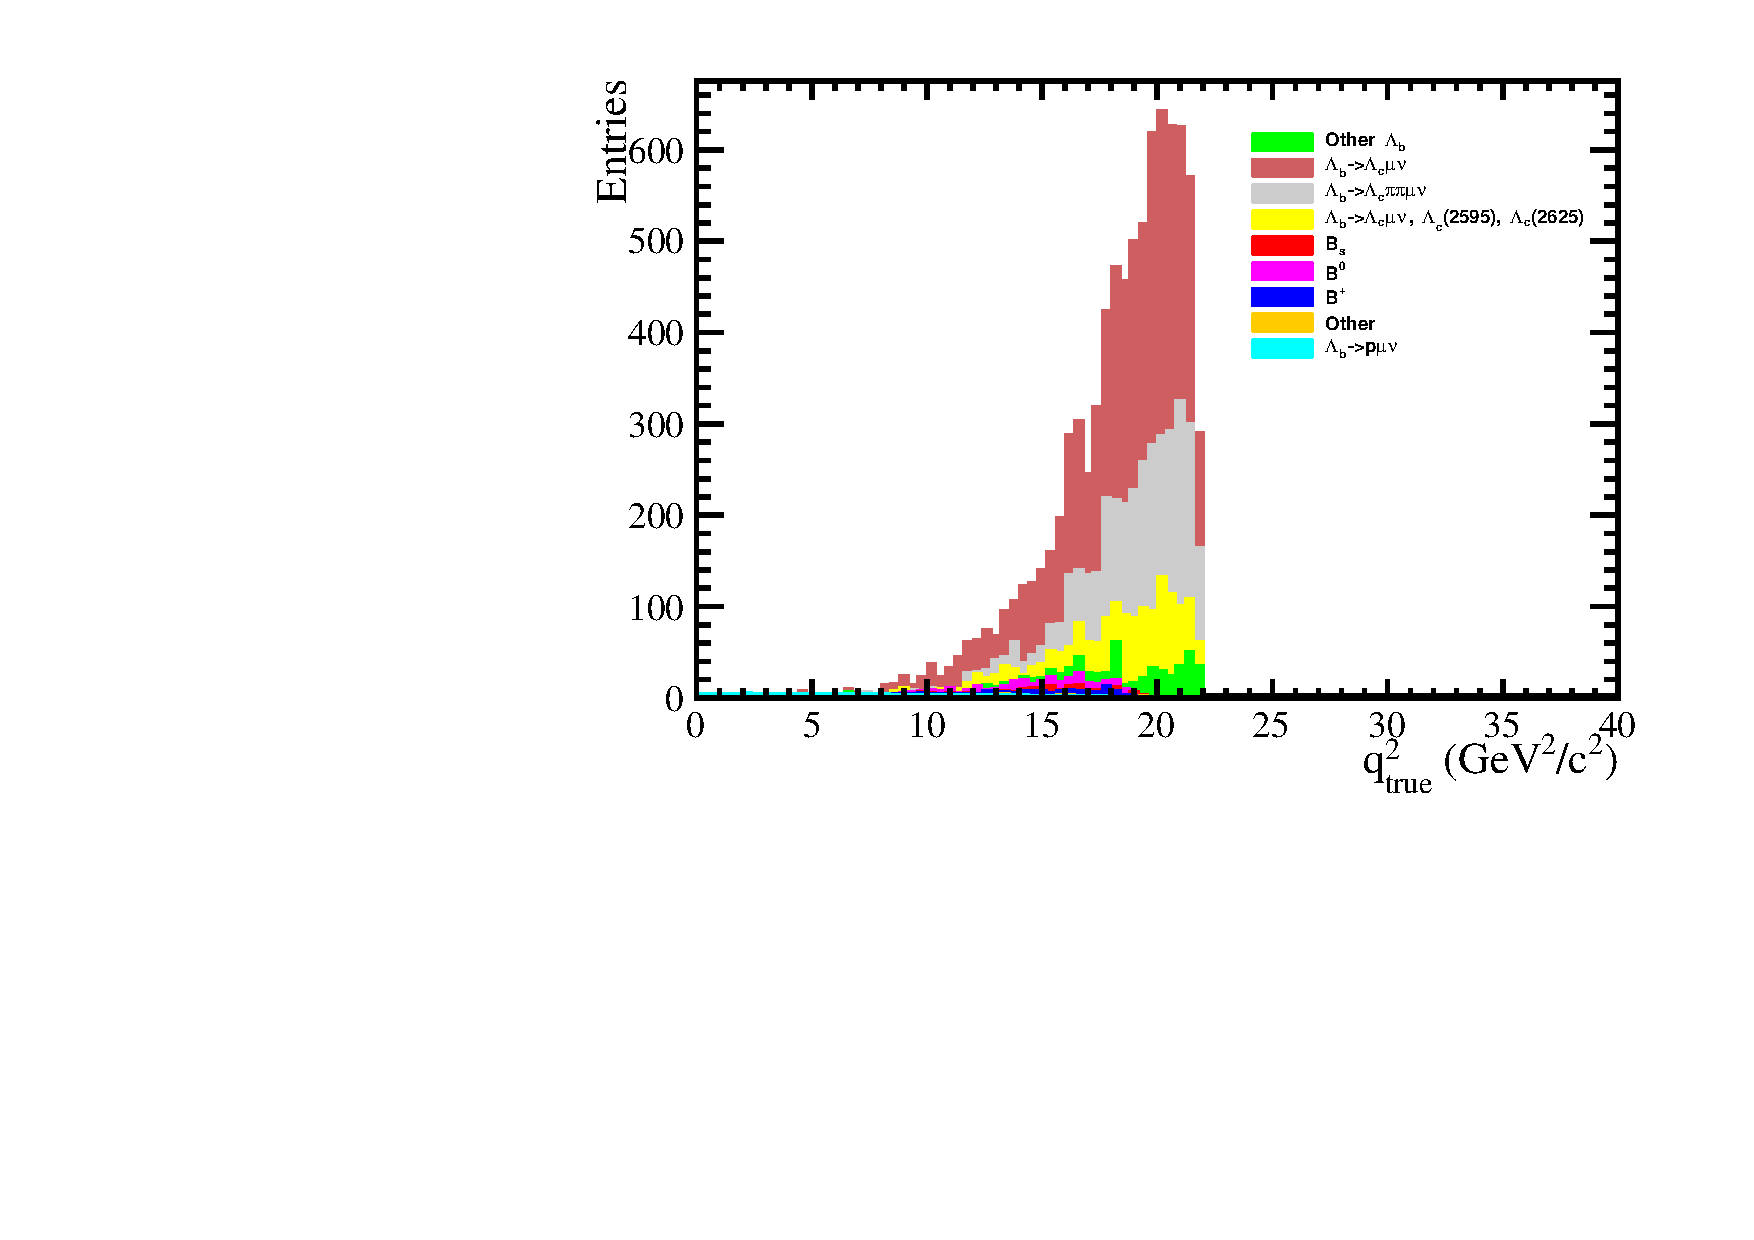
\includegraphics[width=0.8\textwidth]{q2_true_nolog.pdf} 
\end{center}
}

 \frame{
 \frametitle{Opposite Sign $p\mu$ Combinatons}


      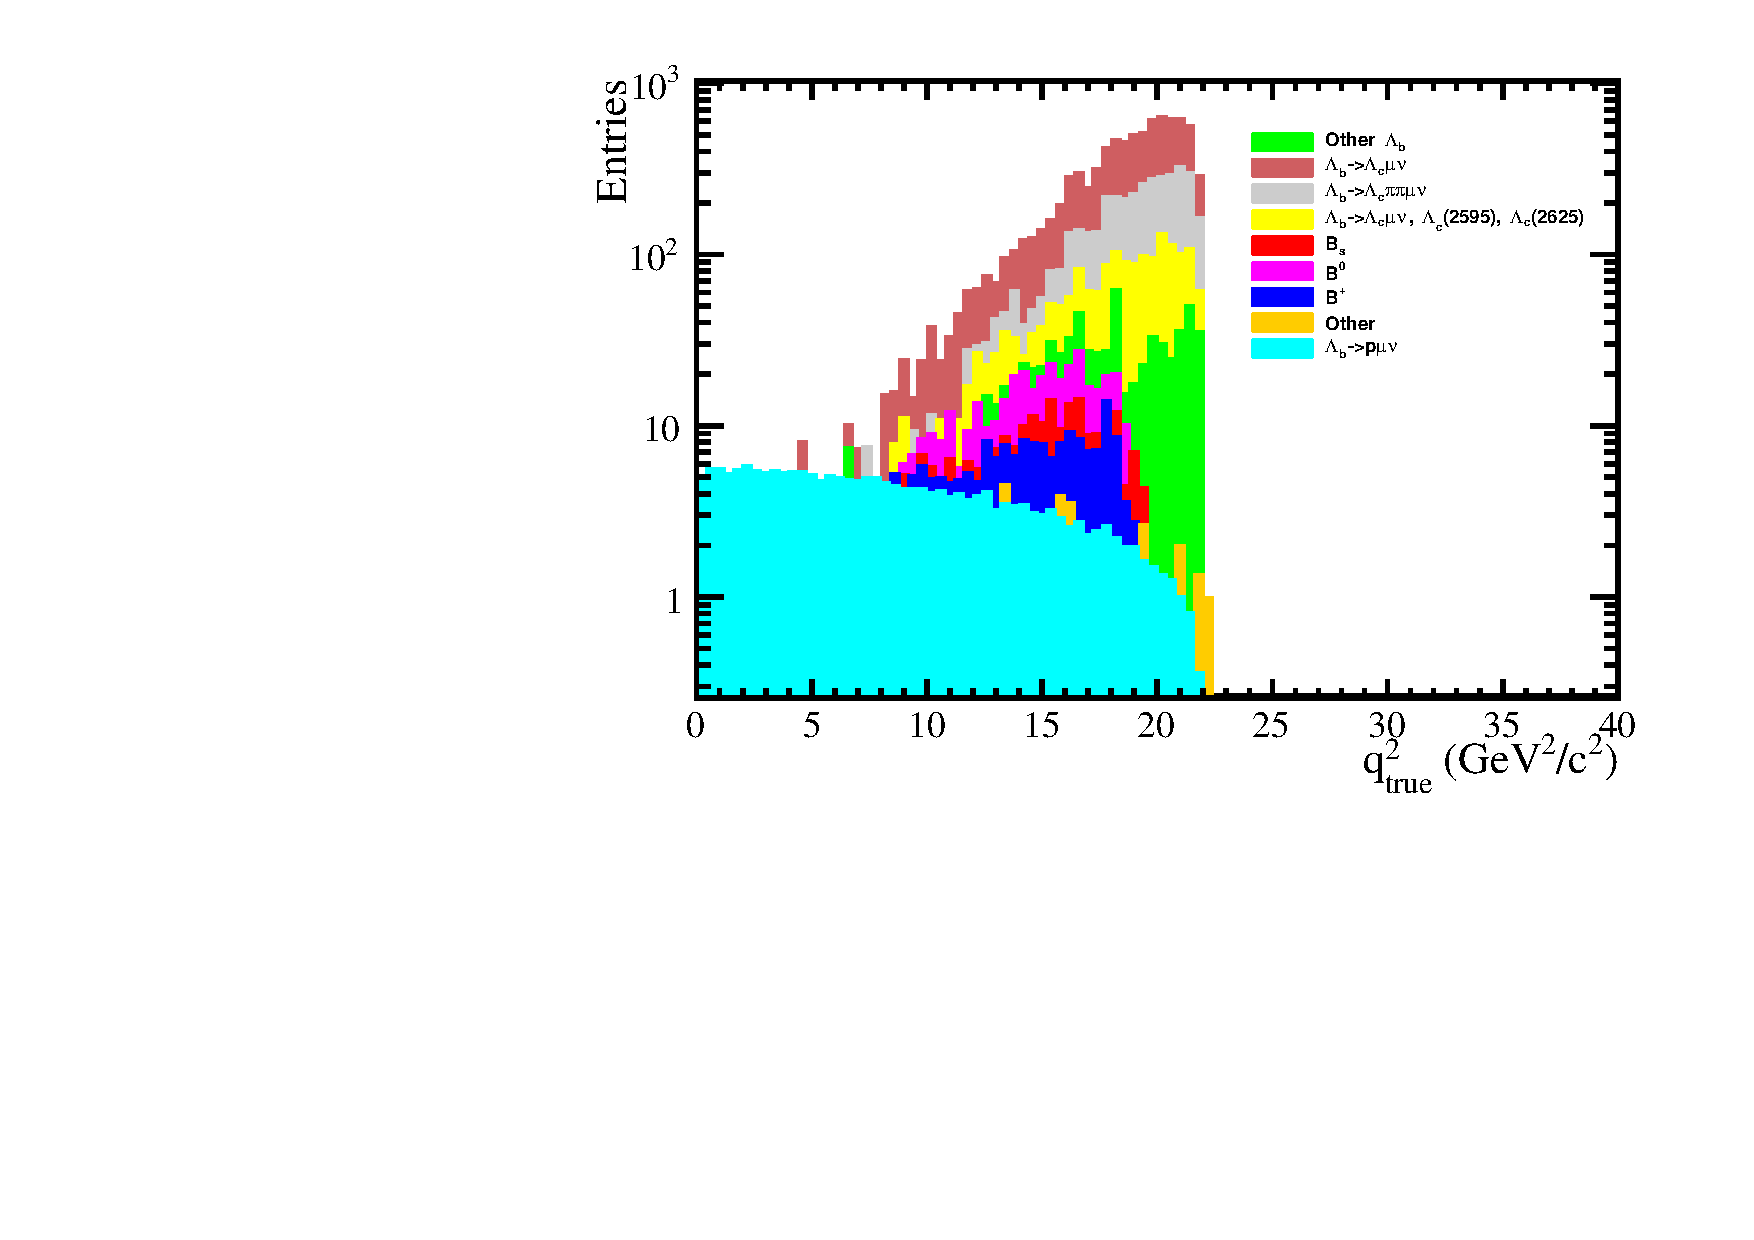
\includegraphics[width=0.5\textwidth]{q2_true_stacked.pdf}    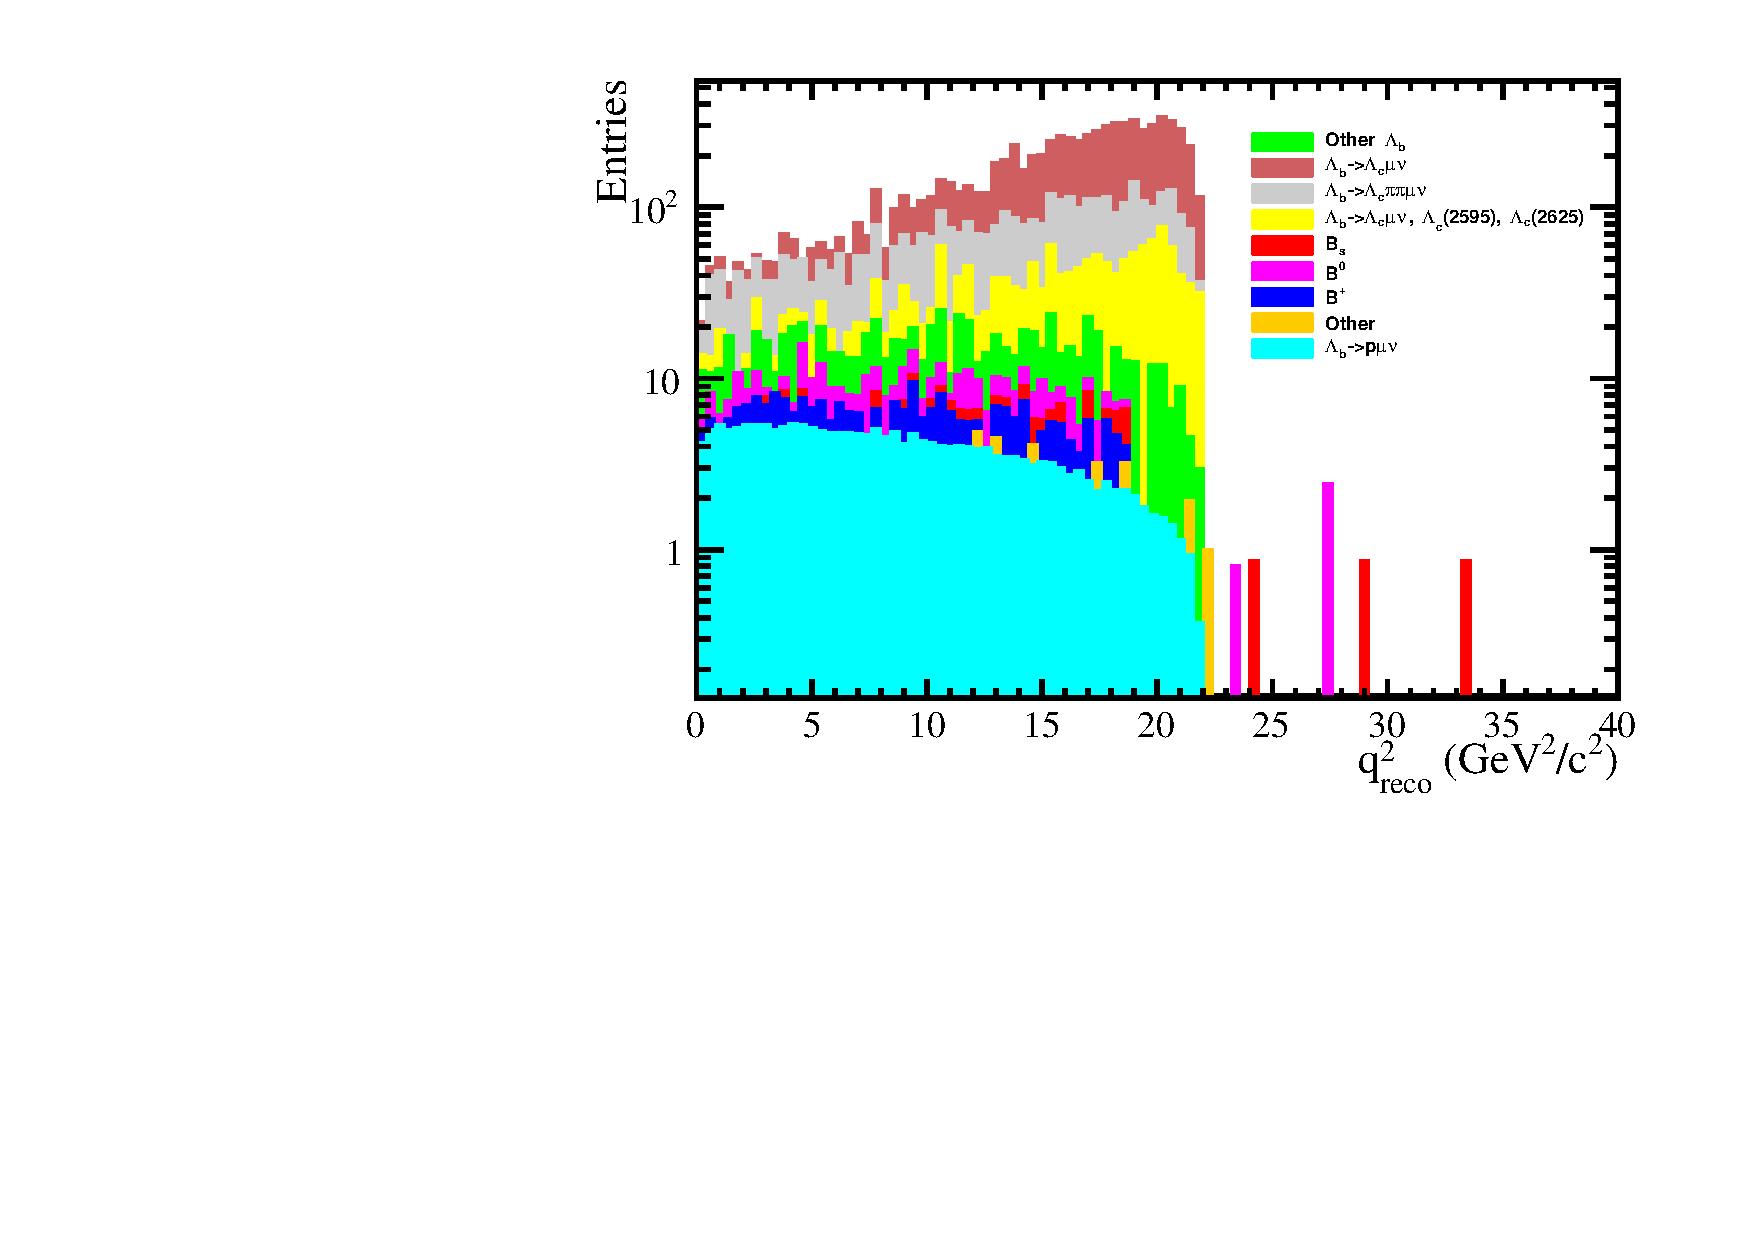
\includegraphics[width=0.5\textwidth]{q2_recon_stacked.pdf} \\
     
       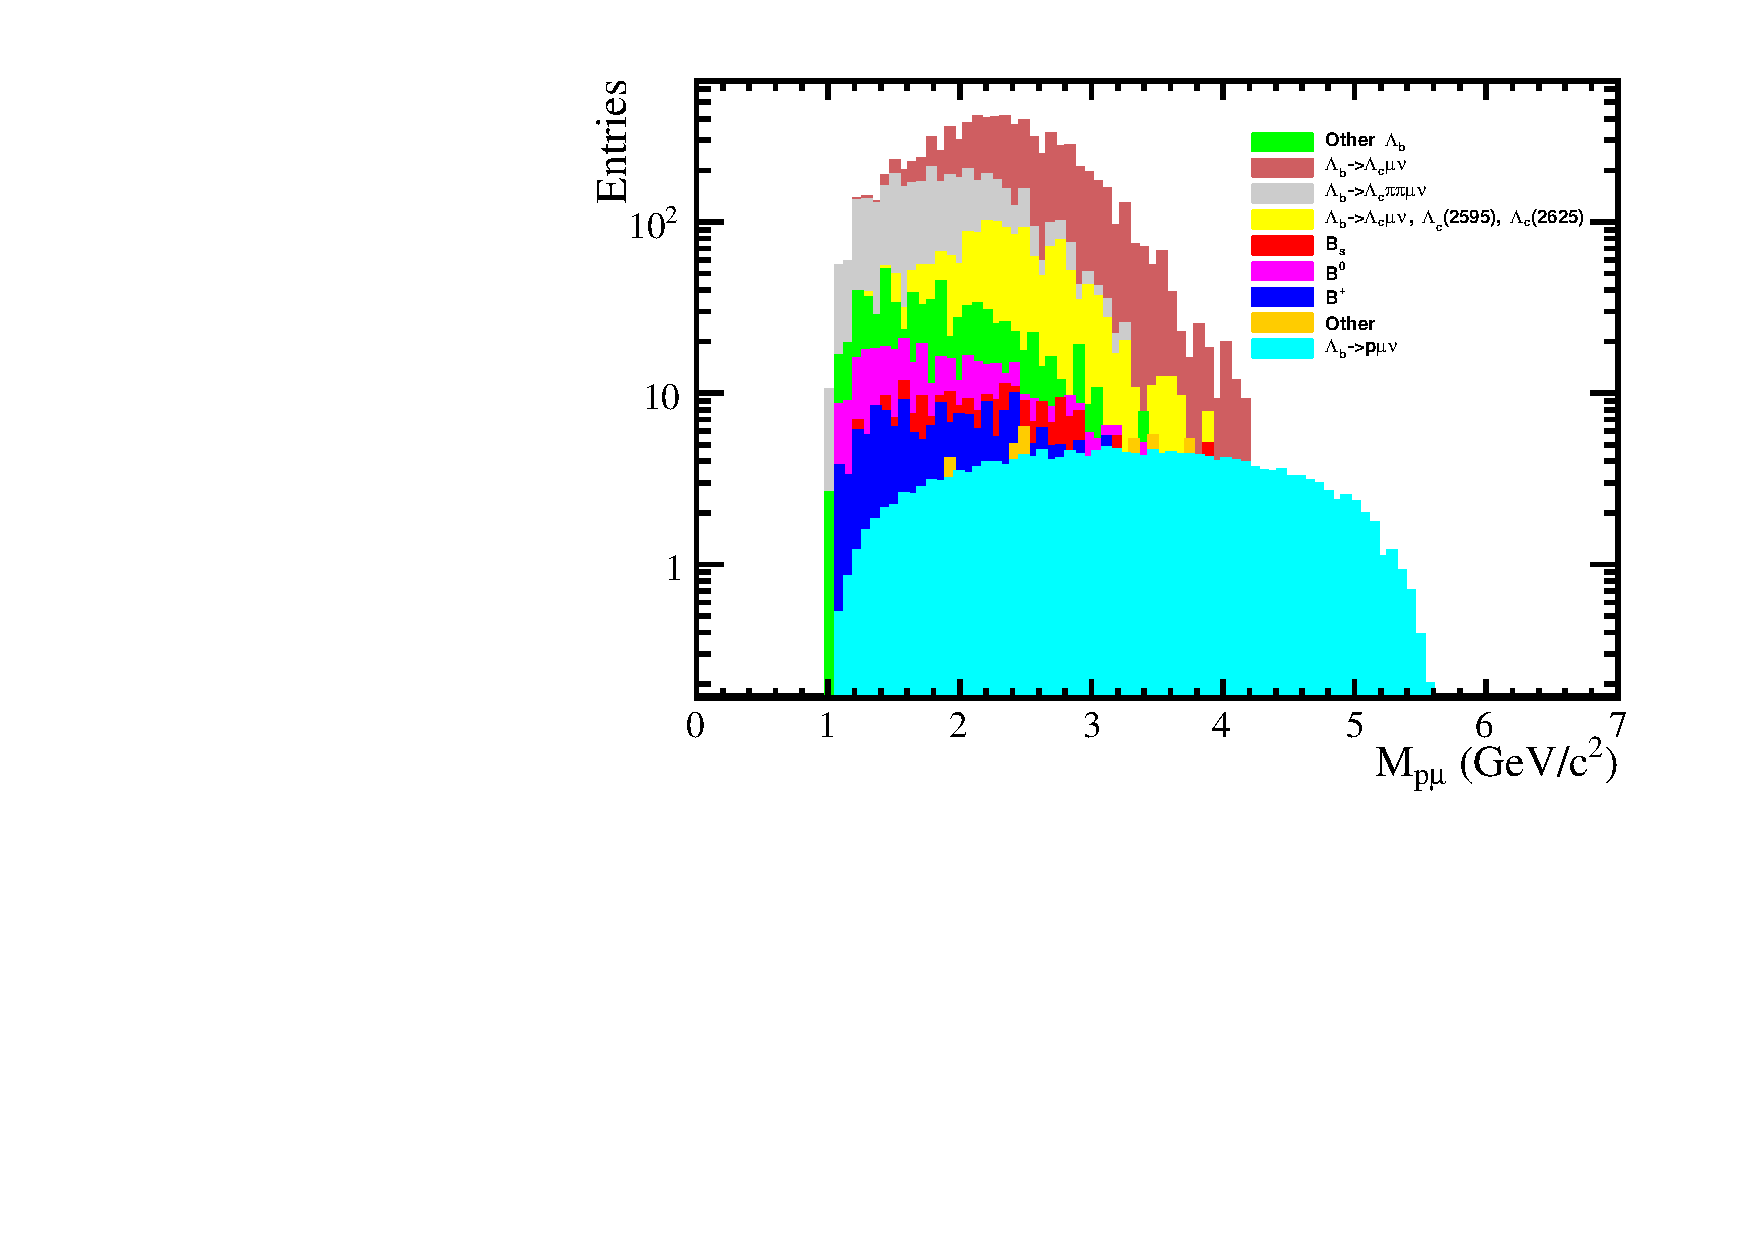
\includegraphics[width=0.5\textwidth]{M_pmu_stacked.pdf}    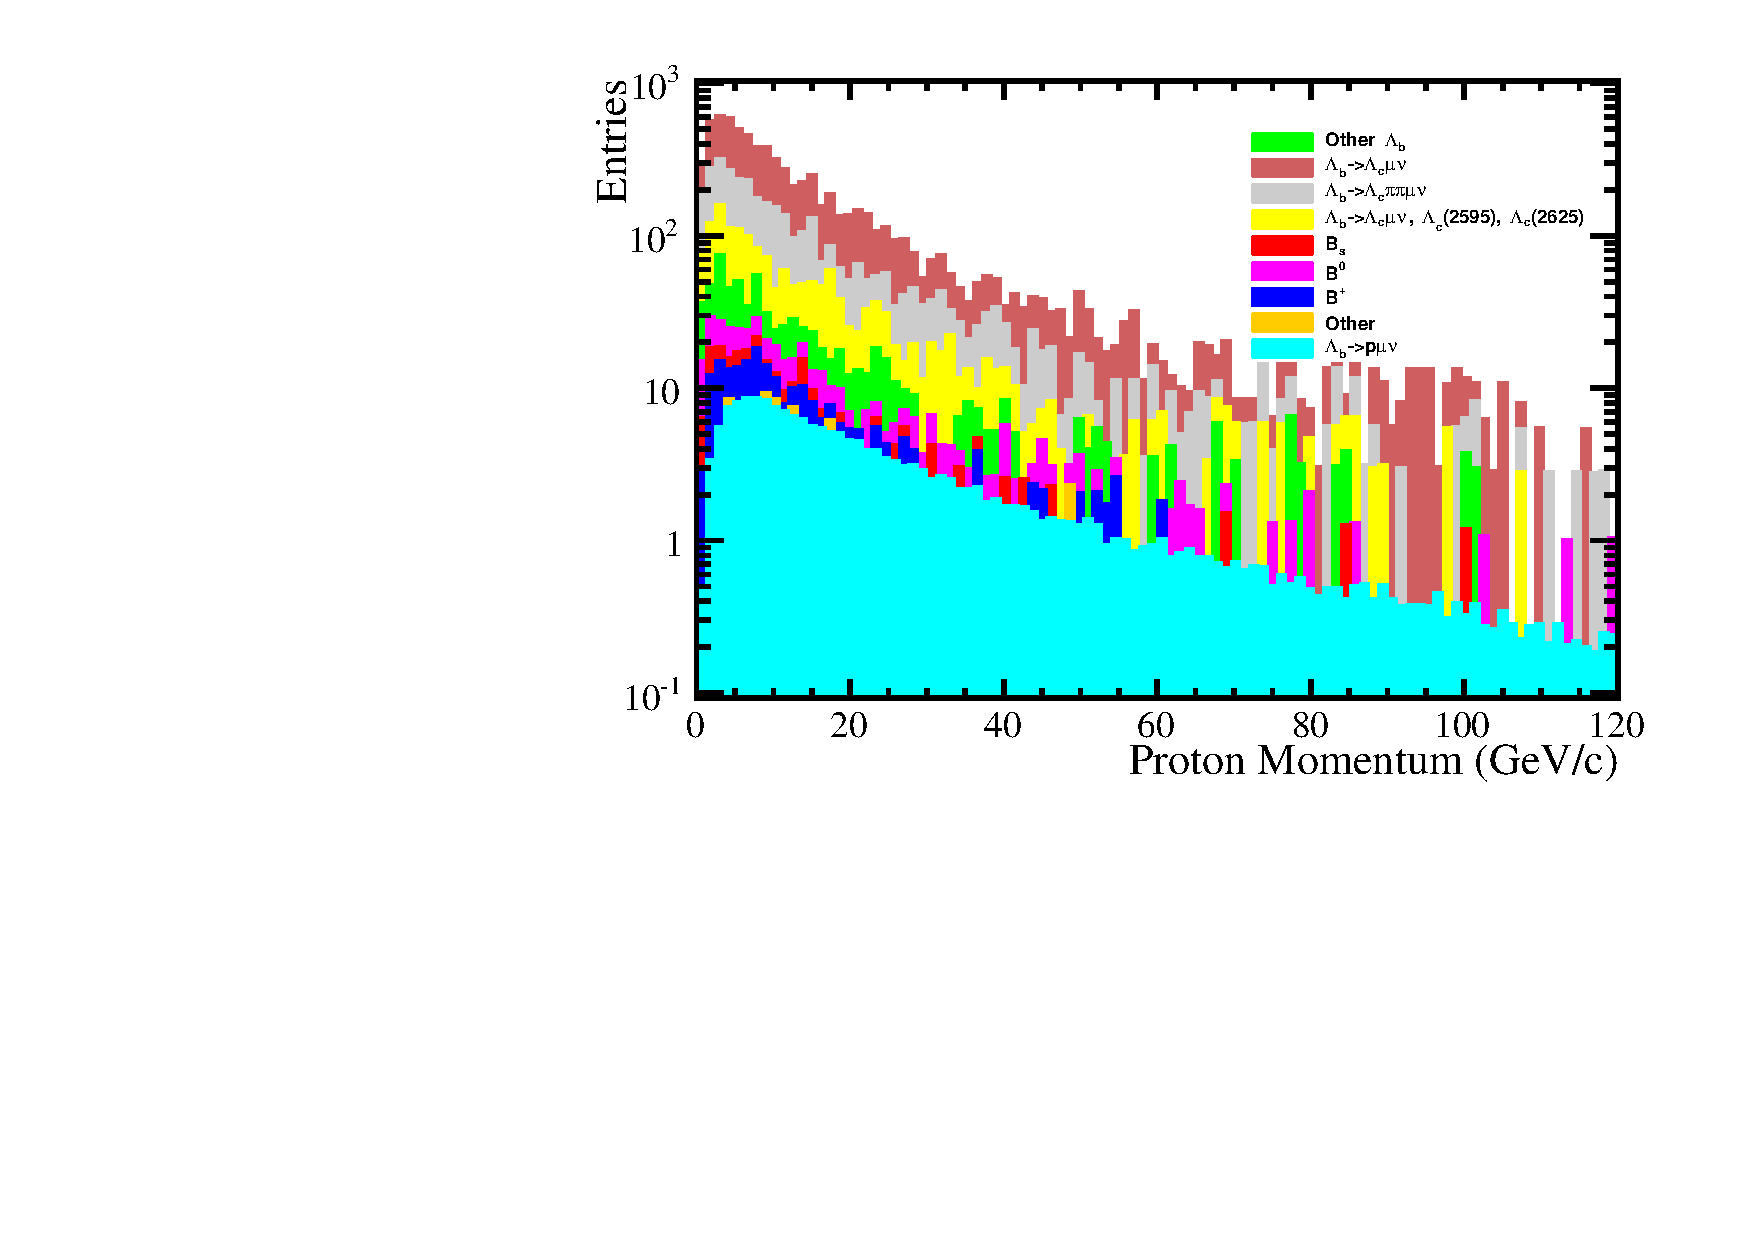
\includegraphics[width=0.5\textwidth]{P_Proton_stacked.pdf} 

}


 
  \frame{
 \frametitle{ Opposite Sign and Same Sign Statistics }
 \begin{itemize}
  \item Find 3391 opposite sign and 716 same sign combinations.
\end{itemize}
\begin{center}
 \hspace{-6cm}  \uline{For Opposite Sign:} \\
 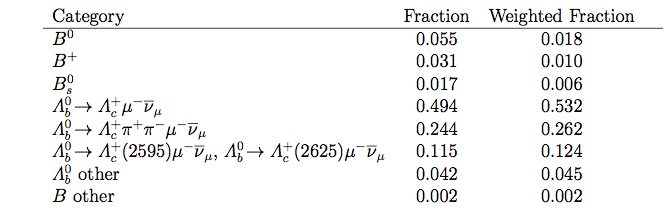
\includegraphics[width=0.75\textwidth]{OS.png}   \\
   \hspace{-6.5cm}  \uline{For Same Sign:} \\
  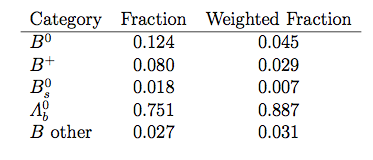
\includegraphics[width=0.4\textwidth]{SS.png}   
  \end{center}
  


}

 \frame{
  \frametitle{Opposite Sign $\pi\mu$ Combinations}
   \begin{itemize}
  \item Can also look for $\pi\mu$ or $K\mu$ combinations.
\end{itemize}
      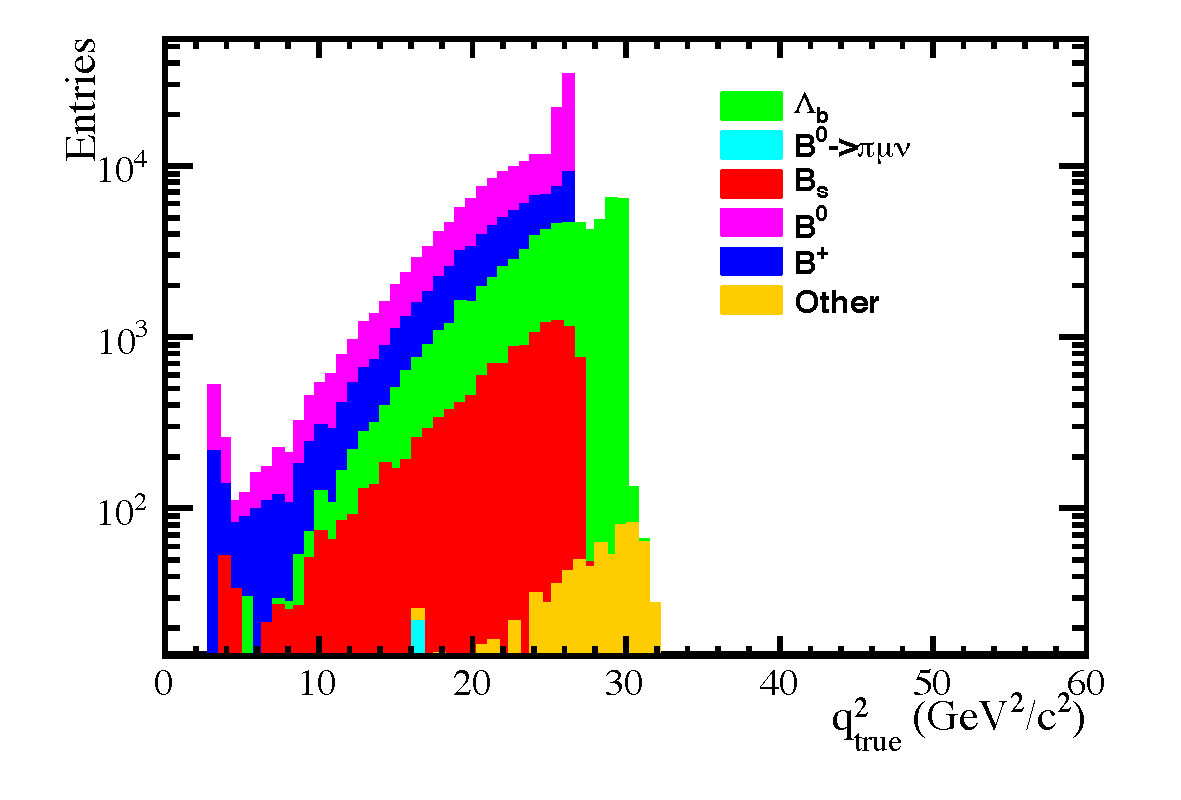
\includegraphics[width=0.45\textwidth]{pimu_q2true_stacked.pdf}    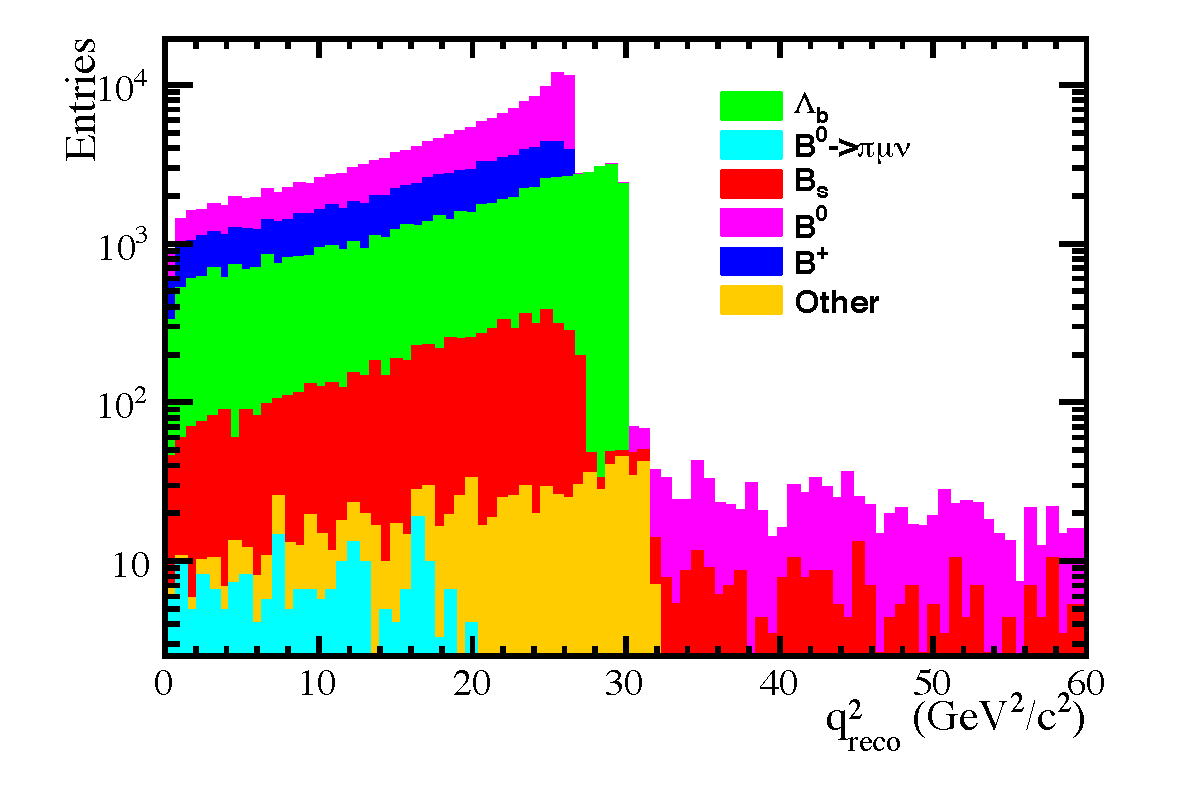
\includegraphics[width=0.45\textwidth]{pimu_q2reco_stacked.pdf} \\
     
       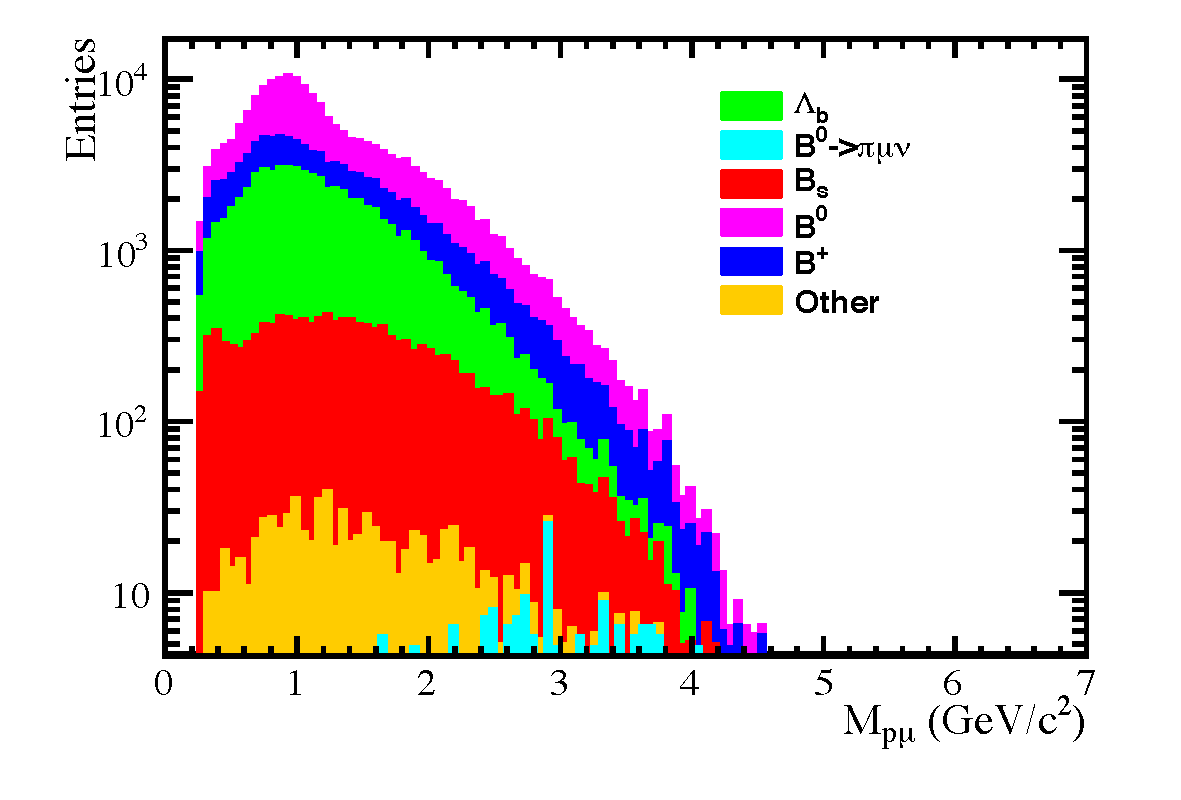
\includegraphics[width=0.45\textwidth]{M_pimu_stacked.pdf}    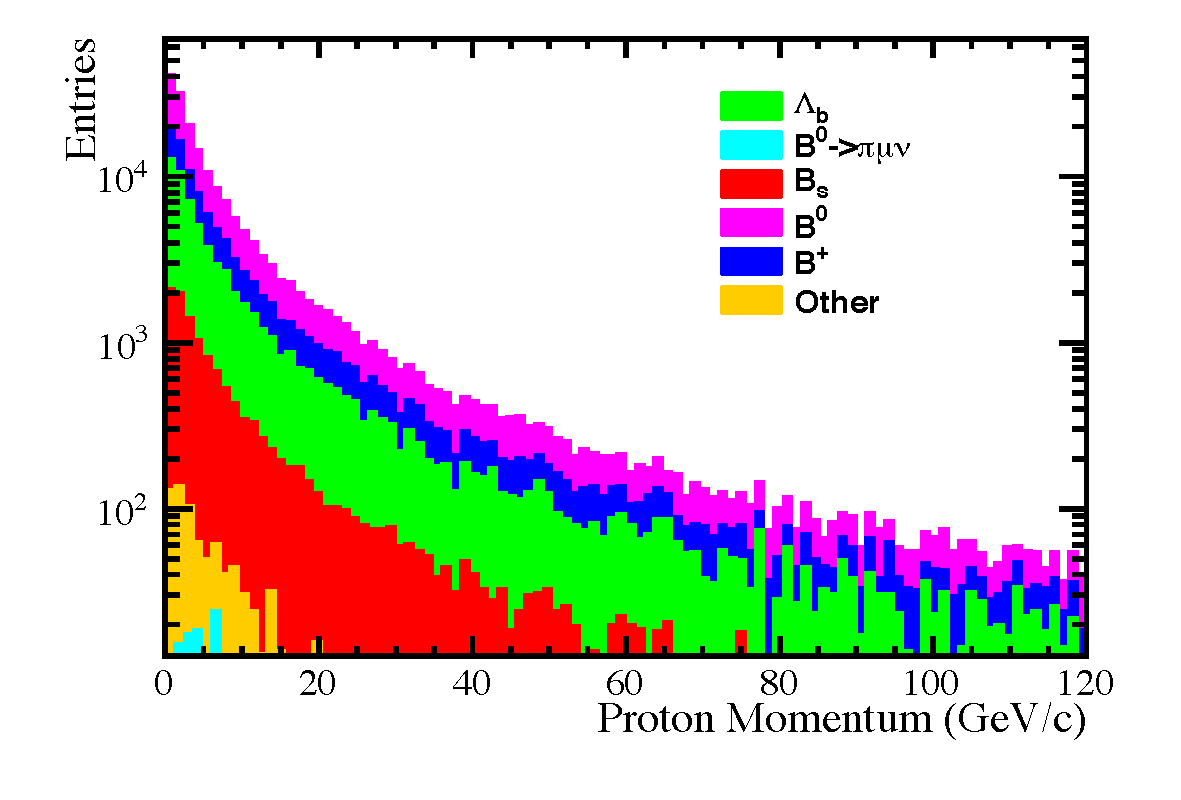
\includegraphics[width=0.45\textwidth]{P_Pion_stacked.pdf} 
}

%%%%%%%%%%%%
\section{Isolation}
 \frame{
 \frametitle{Main backgrounds}
    \begin{itemize}
  \item From generator level studies it is clear that $\Lambda^{0}_{b} \rightarrow \Lambda^{+}_{c} \mu^{-} \overline{\nu}_{\mu}$ is a major background.
  \item This makes sense as branching fraction for $\Lambda^{+}_{c}$ to a proton together with anything  else is $50 \pm 16$\% and $|V_{cb}|^{2}/|V_{ub}|^{2}$$\sim$$100$.
\end{itemize}

\begin{center}
       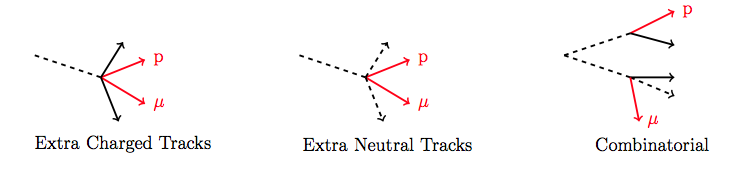
\includegraphics[width=0.9\textwidth]{Isolation1.png}   
       % 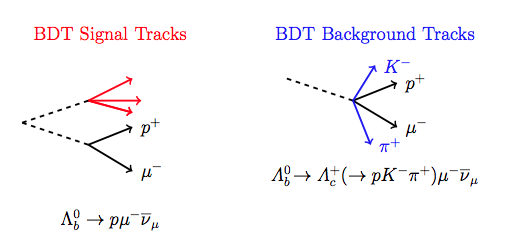
\includegraphics[width=0.45\textwidth]{Isolation2.png} 
       \end{center}

}

  \frame{
 \frametitle{Isolation}
    \begin{itemize}
  \item Train a boosted decision tree to discriminate between charged tracks.
  \item Use following variables: Track $p_{\rm{T}}$, Opening angle, min $\chi^{2}_{IP}$, Ghost Probability,  $\chi^{2}_{IP}$,  Track $\chi^{2}$ and $\chi^{2}_{FD}$.
\end{itemize}
\begin{center}
       %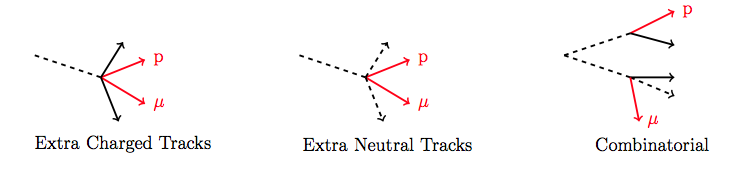
\includegraphics[width=0.9\textwidth]{Isolation1.png}   
        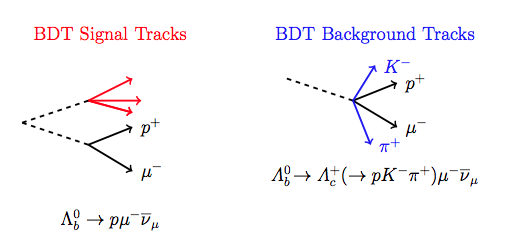
\includegraphics[width=0.8\textwidth]{Isolation2.png} 
       \end{center}
}

  \frame{
 \frametitle{Training Stage}
 
\begin{itemize}
\item Train BDT offline on samples.
  \begin{center}
    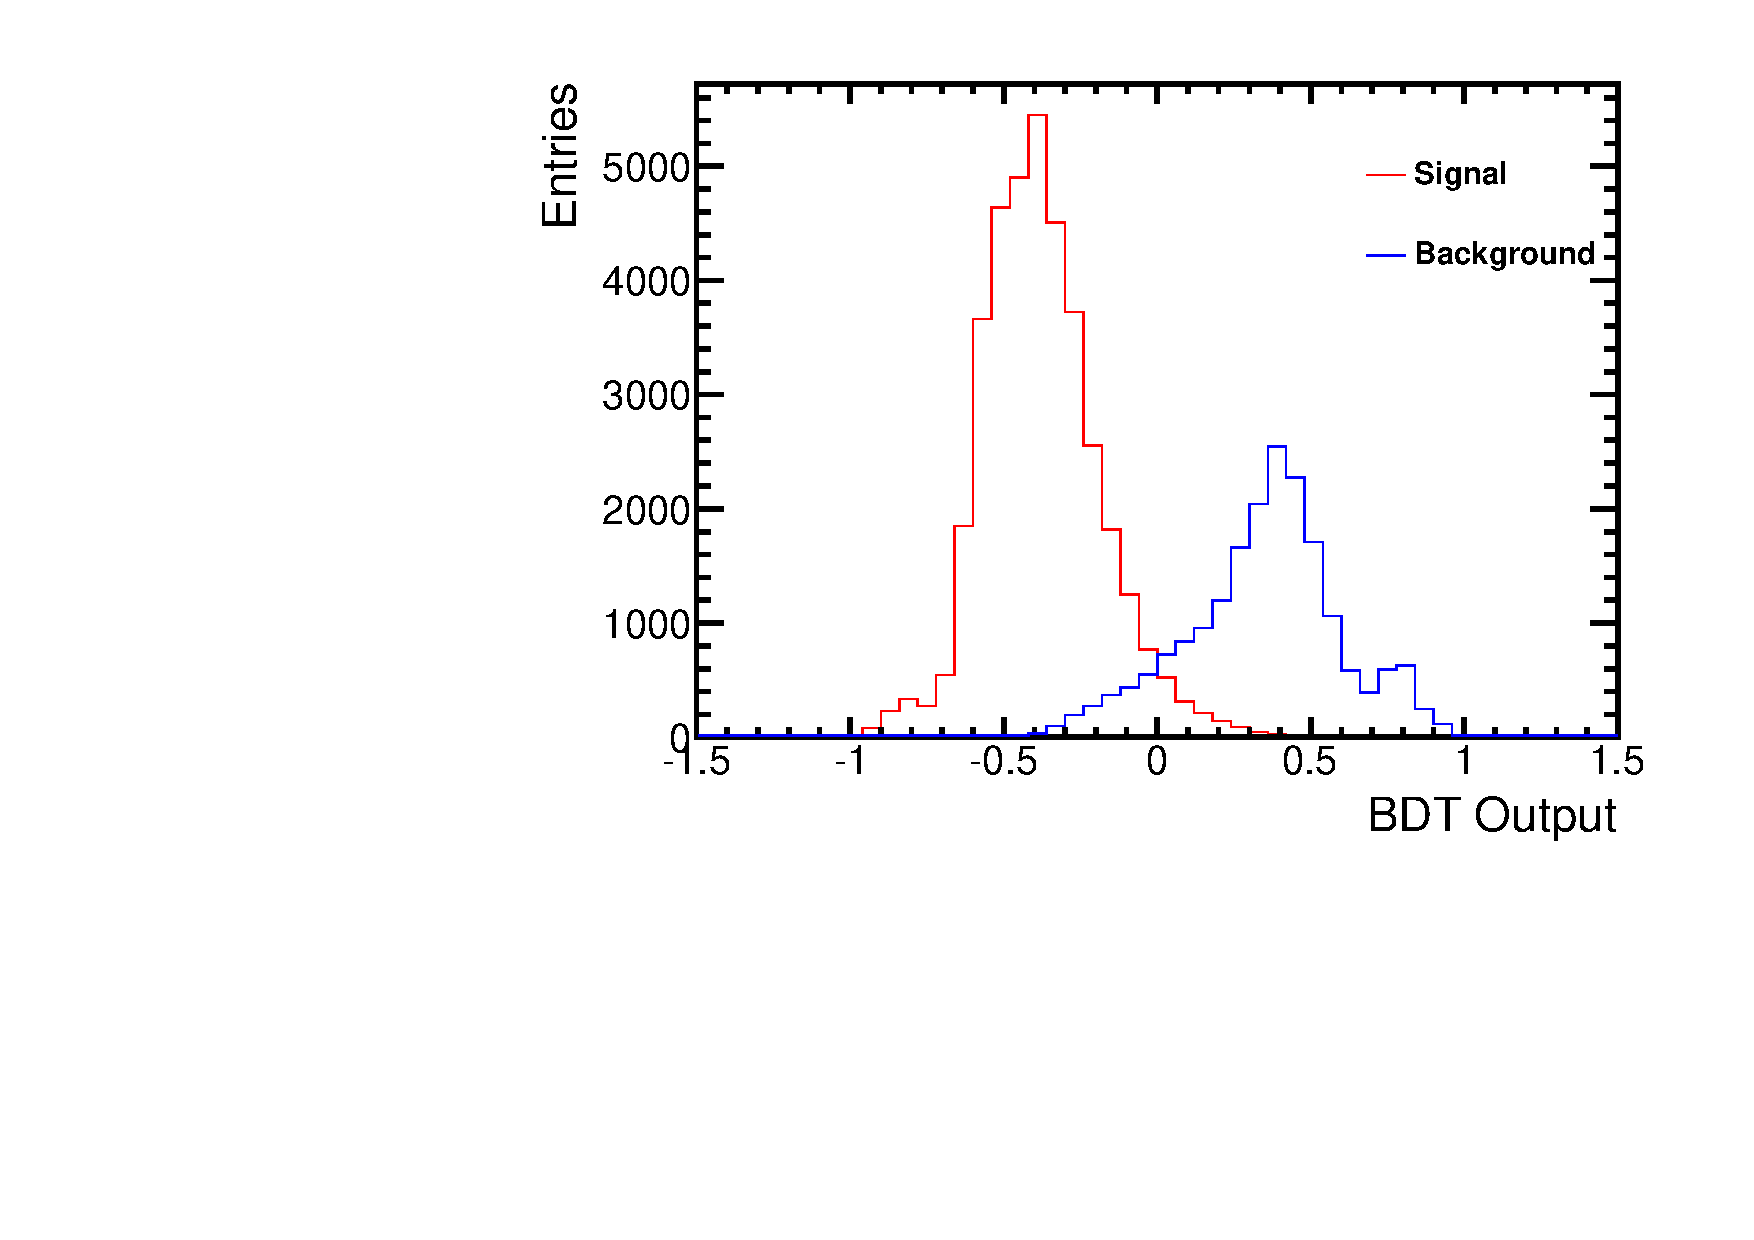
\includegraphics[width=0.8\textwidth]{training.pdf}  
\end{center}

\end{itemize}

}
  \frame{
 \frametitle{Training Stage}
 
\begin{itemize}
\item Run BDT online on all tracks in event. Store maximum BDT output.
  \begin{center}
    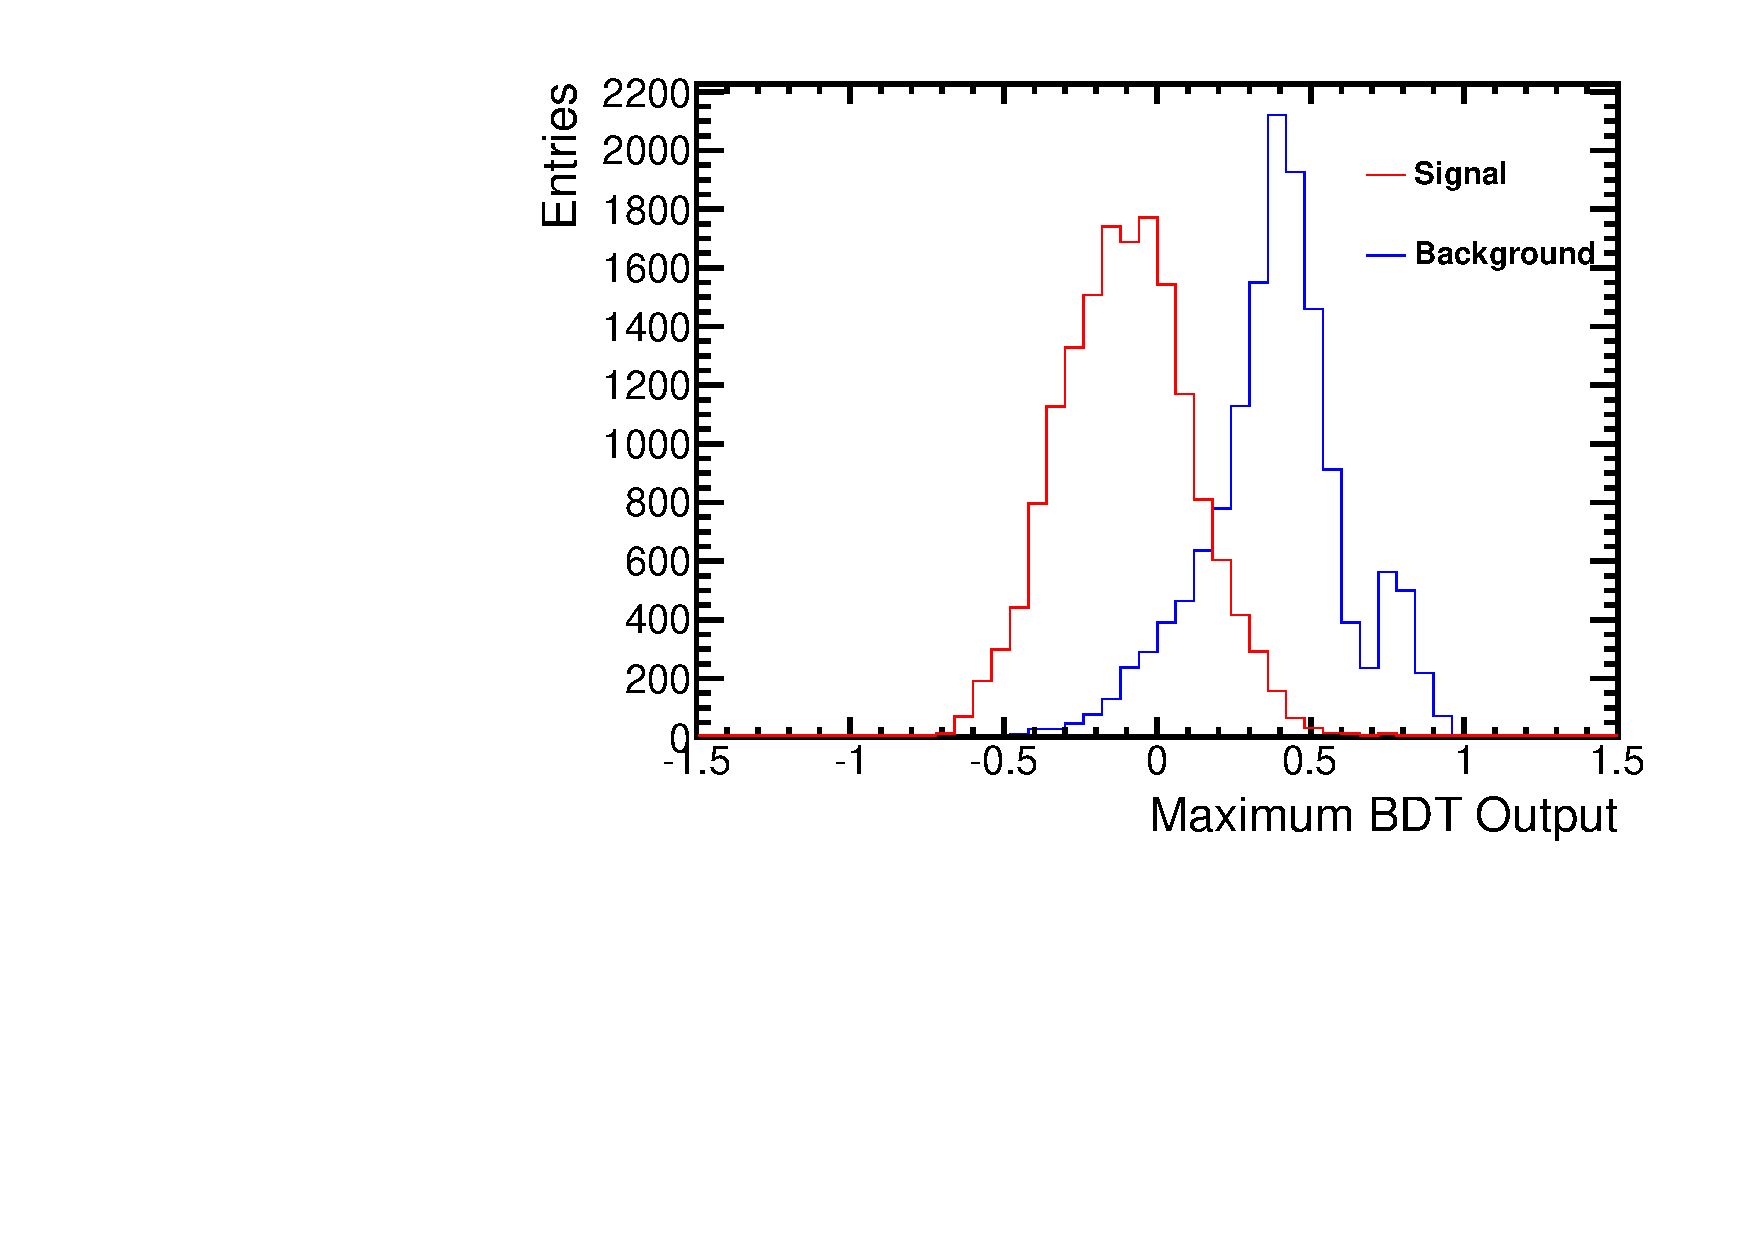
\includegraphics[width=0.8\textwidth]{Isolation_BDT.pdf}  
\end{center}

\end{itemize}

}

%%%%new section
\section{Conclusion}


  \frame{
 \frametitle{Conclusion}
 \begin{itemize}
  \setlength{\itemsep}{5pt}
   \item $E_{\nu}$ cut kills the $q^{2}$ endpoint.
    \item Additional cuts required to reduce rate to 0.5\%.
   \end{itemize}

}

}
 \end{document}